\documentclass{article}

% Pass 'final' to the neurips_2023 package to remove line numbers if needed
\usepackage[final]{neurips_2023}

\usepackage{graphicx}

\usepackage{enumitem}

% \usepackage{placeins}

\usepackage{amsmath}
\usepackage{amsfonts}
\usepackage{bm}

\usepackage[utf8]{inputenc} % allow utf-8 input
\usepackage[T1]{fontenc}    % use 8-bit T1 fonts
\usepackage{hyperref}       % hyperlinks
\usepackage{url}            % simple URL typesetting
\usepackage{booktabs}       % professional-quality tables
\usepackage{amsfonts}       % blackboard math symbols
\usepackage{nicefrac}       % compact symbols for 1/2, etc.
\usepackage{microtype}      % microtypography
\usepackage{xcolor}         % colors

\usepackage{hyperref}
\usepackage{cleveref}

\title{Hybrid UAV Waypoint Tracking Simulation, Results Anlysis and Optimization}

\author{
  Xiaonan (Nice) Wang \thanks{wangxiaonannice@gmail.com} \\
}

\begin{document}

\newcommand{\repeatfootnote}[1]{\textsuperscript{\ref{#1}}}

\maketitle

\begin{abstract}
This document focuses on the simulation results, analysis and corresponding optimizations of ``Hybrid UAV Waypoint Tracking'' simulated by \cite{panerati2021learning}.
\end{abstract}

\section{Mathematical Model}
\subsection{State Space (in 3D space)}
                           
\paragraph{For \textit{Continuous State}:} 
\begin{itemize}
  \item Position: $p\in\mathbb{R}^3$
  \item Velocity: $v\in\mathbb{R}^3$
\end{itemize}

\paragraph{For \textit{Discrete State}:}
\begin{itemize}
  \item Index of Waypoint (Tracking Target): $q\in\mathcal{Q}=\left\lbrace 0,1,2,\dots,N \right\rbrace$
  \begin{itemize}
    \item Coordinates $W=\left\lbrace W_0,W_1,\dots,W_N \right\rbrace$, where $W_q\in\mathbb{R}^3$ is the coordinate of idx $q$
  \end{itemize}
\end{itemize}

Thus, the complete \textbf{hybrid state vector} $\bm{x}$ of the system is defined as:

\begin{equation}
  x = \begin{bmatrix} p \\\ v \\\ q \end{bmatrix} \in \mathbb{R}^6 \times \mathcal{Q}
\end{equation}

\subsection{Flow Set $C$}

The flow set determines the conditions under which the system undergoes continuous-time physical evolution:
\begin{itemize}
  \item As long as the Euclidean distance between the UAV and the current target waypoint $W_q$ is greater than or equal to the tolerance radius $\epsilon$
  \item or if the system has reached the final waypoint ($q=N$), it maintains continuous flight:
\end{itemize}

\begin{equation}
  C = \left\lbrace x \in \mathbb{R}^6 \times \mathcal{Q} \mid \lVert p - W_q \rVert \ge \epsilon \lor q = N \right\rbrace
\end{equation}

\subsection{Flow Map $f$}

Within the flow set, the evolution of the system follows the \textbf{differential equation} $\bm{\dot{x}=f(x)}$. During this phase:

\begin{itemize}
  \item For continuous state:
  \begin{itemize}
    \item $\dot{p} = v$
    \item $\dot{v} = \mathcal{F}_{dyn}(p,v,u_{pid}(p,v,W_q))$
  \end{itemize}
  \item For discrete state $q$: $\dot{q}=0$ since $q$ is invariant in flow set
  \item Physical state is governed jointly by the underlying \textit{rigid body dynamics_ and the _closed-loop PID controller}:
\end{itemize}

\begin{equation}
  \dot{x} = f(x) = \left[ \matrix{ v \\\ \mathcal{F}_{dyn}(p, v, u_{pid}(p, v, W_q)) \\\ 0 } \right], \quad x \in C
\end{equation}

Note:
\begin{itemize}
  \item $u_{pid}$ is the \textit{control command} with $W_q$ acting as the absolute target
  \item $\mathcal{F}_{dyn}$ represents the \textit{rigid body dynamics integration} computed by the underlying \textit{6-DOF physics engine}
\end{itemize}

\subsection{Jump Set ($D$)}

The jump set defines the strict boundary where discrete events (\textit{transients})  are triggered:
\begin{itemize}
  \item When the UAV enters the $\epsilon$-neighborhood of the target waypoint
  \item and the current waypoint is not the final destination
\end{itemize}

The state machine triggers a jump:

\begin{equation}
  D = \left\lbrace x \in \mathbb{R}^6 \times \mathcal{Q} \mid \lVert p - W_q \rVert < \epsilon \land q < N \right\rbrace
\end{equation}

\subsection{Jump Map ($g$) (\textit{i.e. Transition})}

When the state $x\in D$, the system undergoes a discrete jump $x^+=g(x)$. 
\begin{itemize}
  \item At this instant, the physical position and velocity remain continuous (\textbf{no spatial mutation occurs})
  \item but the target waypoint index $q$ advances to the next one:
\end{itemize}

\begin{equation}
  x^+=g(x)=\begin{bmatrix}p\\\v\\\q+1\end{bmatrix},\quad x\in D
\end{equation}

\subsection{Overall Hybrid Automaton Equations}

\begin{equation}
  \mathcal{H} := \begin{cases} 
    \dot{x}=f(x),&x\in C \\\ x^+=g(x),&x\in D 
  \end{cases}
\end{equation}

\section{Simulation Results}
\subsection{Initial Exp}

\paragraph{State \& Trajectory Plot} The initial experiment's state plot and trajectory plot see \cref{fig:state} and \cref{fig:traj}.

\begin{figure}[tb]
  \centering
  
\includegraphics[width=0.95\textwidth]{fig/state.png}
  \caption{Initial Exp: State Plot}
  \label{fig:state}
\end{figure}

\begin{figure}[tb]
  \centering
  
\includegraphics[width=0.95\textwidth]{fig/traj.png}
  \caption{Initial Exp: Trajectory Plot}
  \label{fig:traj}
\end{figure}

\subsection{Simulation Results Analysis}

\paragraph{Conclusion:} The breakdown of local stability in \textbf{underactuated systems} under large step inputs.

\paragraph{Overview Results Analysis:} As observed in the state and trajectory plots, the UAV successfully tracks the initial waypoints, indicated by the discrete mode transitions ($q = 0 \to 1 \to 2$). However, upon switching to mode $q=2$ (targeting [2.0, 2.0, 1.5]), the large spatial distance introduces a severe step-error to the closed-loop controller. This forces an aggressive attitude adjustment, evident from the violent high-frequency oscillations in the Orientation plot (Roll/Pitch/Yaw) after $t \approx 2s$. The extreme tilt angles cause the vertical thrust component to drop below gravity ($T\cos\theta < mg$), leading to an irreversible altitude loss ($Z \to 0$, as seen in the Position plot). The UAV hits the ground and becomes locked in an unrecoverable physical state, failing to ever enter the $\epsilon$-neighborhood (Jump Set $D$) of the subsequent waypoint. Consequently, the discrete state $q$ permanently stalls at 2.

\paragraph{Potential Dynamical Properties to Study:} 
\begin{itemize}
  \item \textbf{Stability (Region of Attraction):} The continuous flow map $f(x)$ utilizing standard PID control is only \textit{locally asymptotically stable} for \textbf{the 6-DOF underactuated system}. It exhibits severe instability under large step inputs due to the coupling between attitude and translational dynamics.
  \item \textbf{Attractivity (Reachability):} The target jump set $D_{q+1}$ is not attractive from the post-jump initial state $x(t_0)$ under the current flow map. The continuous trajectory diverges to the ground singularity before intersecting $D$.
  \item \textbf{Robustness:} The current system architecture lacks robustness against actuator saturation (motor RPM limits) and unmodeled ground-effect disturbances when subjected to extreme attitude commands.
\end{itemize}

\paragraph{Outline of a Possible Analysis Approach:} 
\begin{itemize}
  \item \textbf{Step 1: Lyapunov-based Stability Analysis:} Construct a Control Lyapunov Function (CLF), denoted as $V(x)$, for the closed-loop continuous dynamics to estimate the \textbf{Maximum Region of Attraction (ROA)} regarding the allowable positional tracking error.
  \item \textbf{Step 2: Forward Reachability Verification:} Mathematically verify whether the initial state immediately following a discrete jump, $x^+ = g(x)$, safely resides within the established ROA of the subsequent flow map.
  \item \textbf{Step 3: Trajectory Redesign (Controller Synthesis):} Introduce a sufficiently smooth reference trajectory planner (e.g., a minimum-snap or cubic polynomial interpolator) into $f(x)$. This ensures the instantaneous tracking error remains strictly bounded within the ROA, guaranteeing forward invariance and successful intersection with all subsequent jump sets.
\end{itemize}

\subsection{Optimization Exp}

\paragraph{Optimizations}
\begin{itemize}
  \item \textbf{Virtual Target Initialization:} Introduced a `virtual_target_pos` state variable initialized exactly at the drone's spawn location:
  \begin{itemize}
    \item This ensures the \textbf{initial control error is zero},
    \item \textbf{preventing any violent takeoff maneuvers}.
  \end{itemize}
  \item \textbf{Kinematic Trajectory Generator (Linear Interpolation):} Added a \textbf{smooth interpolation mechanism} \textit{inside} the continuous Flow Map $f(x)$ loop. Instead of instantly switching to the next distant waypoint, the virtual target moves towards the absolute waypoint at a \textbf{constrained, constant velocity} (MAX_SPEED = 0.8 m/s). -> Enhance Stability
  \item \textbf{Elimination of Step-Inputs for the Controller:}
  \begin{itemize}
    \item Modify the PID controller to track this continuously moving `virtual_target_pos` rather than the absolute `WAYPOINTS[q]`.
    \item By breaking down the large spatial gap into millimeter-level, time-stepped increments, we completely eliminated the massive step-errors that previously caused extreme attitude (pitch/roll/yaw) oscillations and the local stability failure of the underactuated system.
  \end{itemize}
\end{itemize}

\paragraph{State \& Trajectory Plot \& GUI Display} The optimization experiment's state plot, trajectory plot and gui display see \cref{fig:state_opt}, \cref{fig:traj_opt} and \cref{fig:gui_opt}.

\begin{figure}[tb]
  \centering
  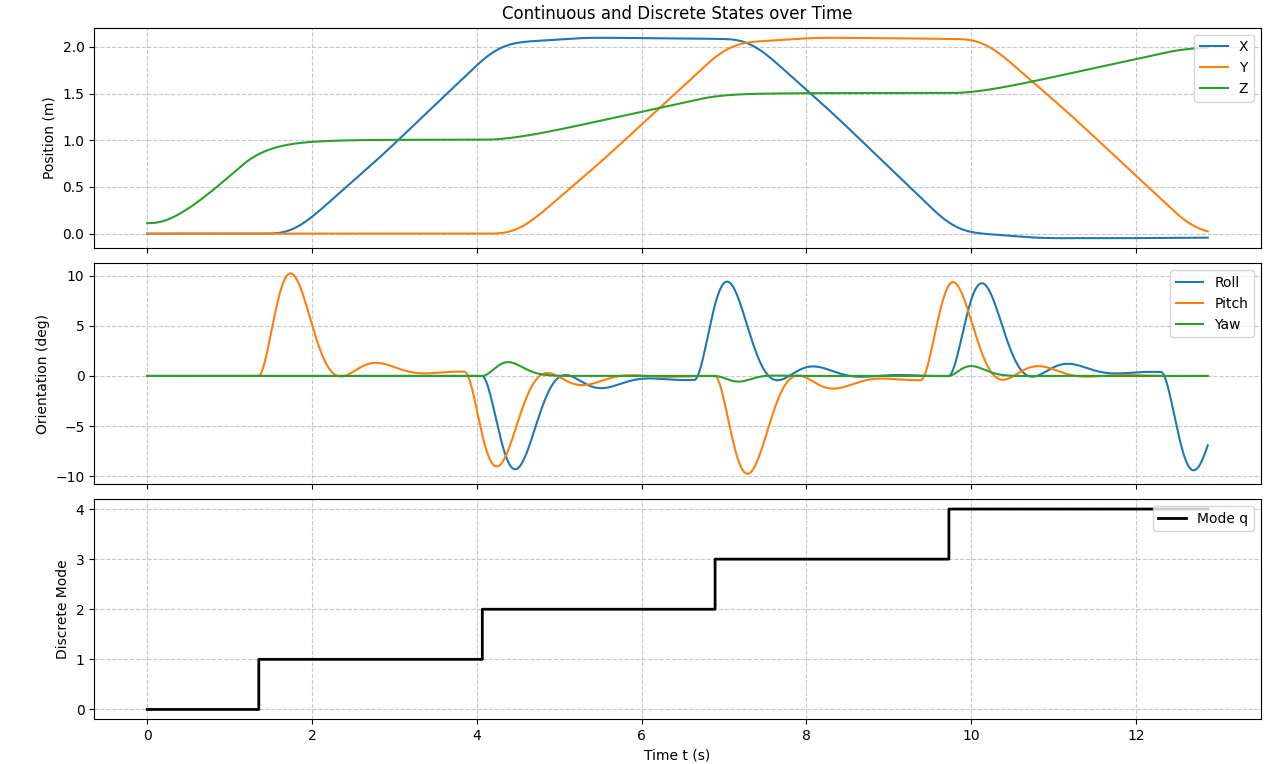
\includegraphics[width=0.95\textwidth]{fig/state_opt.png}
  \caption{Optimization Exp: State Plot}
  \label{fig:state_opt}
\end{figure}

\begin{figure}[tb]
  \centering
  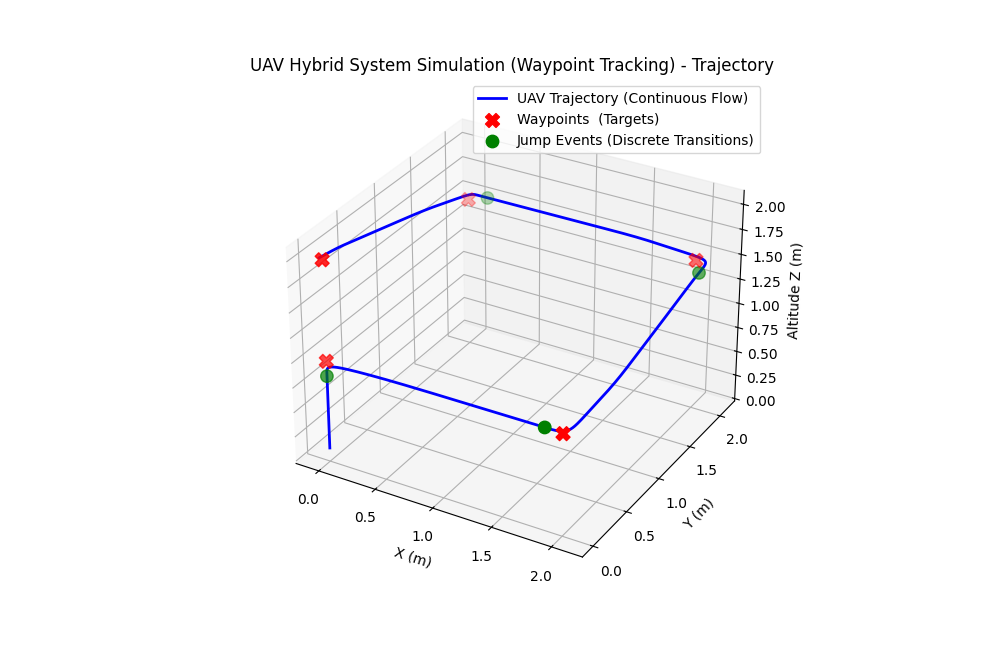
\includegraphics[width=0.95\textwidth]{fig/traj_opt.png}
  \caption{Optimization Exp: Trajectory Plot}
  \label{fig:traj_opt}
\end{figure}

\begin{figure}[tb]
  \centering
  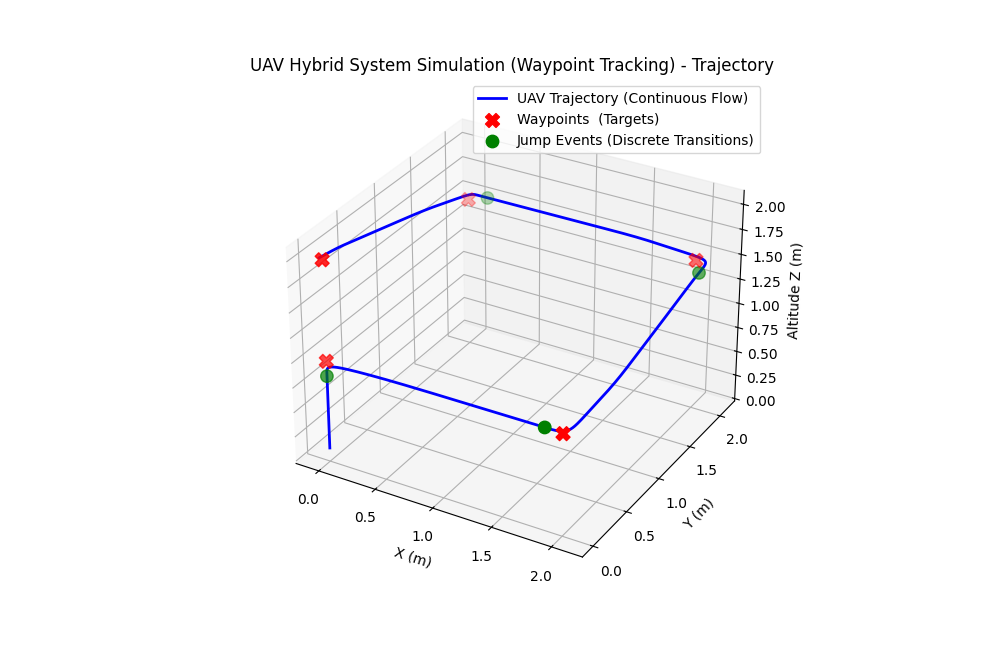
\includegraphics[width=0.95\textwidth]{fig/traj_opt.png}
  \caption{Optimization Exp: Simulation GUI Display}
  \label{fig:gui_opt}
\end{figure}

\bibliographystyle{abbrvnat}
\bibliography{main}
\end{document}
